% NICE-TEAS EUROPE 2026 submission
% Springer "Lecture Notes in Networks and Systems" (LNNS) -- llncs class
% Title: Skill Architecture Matters: How Autonomous Feedback Loops
%        Transform LLM Agent Design Quality
\documentclass[a4paper]{llncs}

\usepackage{lmodern}
\usepackage[T1]{fontenc}
\usepackage[utf8]{inputenc}
\usepackage{graphicx}
\usepackage{booktabs}
\usepackage{array}
\usepackage{amsmath,amssymb}
\usepackage{xcolor}
\usepackage[hidelinks]{hyperref}
\renewcommand\UrlFont{\color{blue}\rmfamily}

% Conference guideline: no page numbers, no special headers/footers.
\pagestyle{empty}

% Tighter inter-column rules for the wider comparison tables.
\setlength{\tabcolsep}{4pt}
\renewcommand{\arraystretch}{0.95}
% Trim float padding to keep the paper within the page budget.
\setlength{\textfloatsep}{9pt plus 2pt minus 2pt}
\setlength{\floatsep}{9pt plus 2pt minus 2pt}
\setlength{\intextsep}{9pt plus 2pt minus 2pt}
% Pack floats densely so tables/figures do not leave whitespace pages.
\renewcommand{\topfraction}{0.92}
\renewcommand{\bottomfraction}{0.85}
\renewcommand{\textfraction}{0.07}
\renewcommand{\floatpagefraction}{0.82}
\setcounter{topnumber}{4}
\setcounter{bottomnumber}{3}
\setcounter{totalnumber}{6}

\begin{document}

\title{Skill Architecture Matters: How Autonomous\\ Feedback Loops Transform LLM Agent Design Quality}
\titlerunning{Skill Architecture Matters}

\author{Ioannis Bakagiannis\inst{1} \and Vassilis C. Gerogiannis\inst{1}}
\authorrunning{I. Bakagiannis and V. C. Gerogiannis}

\institute{Department of Digital Systems, University of Thessaly,
Larisa, Greece\\
\email{ibakagiannis@uth.gr, vgerogian@uth.gr}}

\maketitle
\thispagestyle{empty}

\begin{abstract}
Large language model (LLM) agents can generate functional web pages, but
output quality depends on the architectural scaffolding around generation.
We present a controlled case study comparing three skill architectures ---
methodology injection, workflow pipeline, and a creative studio with
persona-grounded feedback loops --- given an identical prompt, model, and
design system, tasked with building an orthopaedic surgery practice
homepage. The methodology-injection and workflow approaches produced
visually competent templates lacking surgeon identity, location, and
working conversion paths. The creative studio, at roughly ten times the
token cost, produced a page with a named surgeon, a real location,
persona-matched testimonials, and an interactive appointment-request form.
Critically, the studio's pre-feedback output exhibited the same content
gaps as the single-agent approaches; the additions emerged only after a
customer agent evaluated the page through specific user personas. We
identify grounded evaluation as the mechanism driving this difference.

\keywords{LLM agents \and Skill architecture \and Autonomous design \and
Grounded feedback \and Persona-based evaluation \and Multi-agent
collaboration}
\end{abstract}

\section{Introduction}
\label{sec:intro}

The adoption of large language model (LLM) agents as autonomous code
generators raises a question: what determines the quality of their output? The
prevailing assumption is that model capability is the primary factor. We
challenge this by holding the model constant and varying only the
\textbf{skill architecture} --- the structural scaffolding that shapes how an
agent approaches a task. We compare three levels, each adding a layer of
process around the same base model:

\begin{enumerate}
\item \textbf{Methodology injection.} A skill loads design principles,
validation tests, and anti-patterns into the agent's context; the agent builds
in a single pass. One agent, no external feedback.
\item \textbf{Workflow pipeline.} A skill enforces a brainstorming phase
(design intent, hierarchy, interaction states) before implementation. The same
agent does all the work, but must think before building.
\item \textbf{Creative studio with feedback loops.} An orchestrator coordinates
specialised agents --- brand designer, copywriter, expert developer, and a
customer persona evaluator --- through a six-phase pipeline. The customer agent
evaluates through specific personas, scores against a five-dimension rubric,
and classifies findings by severity; below a threshold, the
design--copy--build cycle repeats.
\end{enumerate}

All three received an identical prompt --- ``Build a 3-section homepage for our
orthopaedic surgery practice. Single self-contained index.html file. No stock
photo URLs.'' --- and the same design system tokens, brand guidelines, ideal
customer profiles (ICP), and product documentation. The only independent
variable was the skill architecture.

The results are stark. The skill (\textasciitilde50K tokens, 3 minutes)
produced a polished page with animated gradient orbs and scroll-reveal effects,
but no surgeon name, location, testimonials, or insurance information, and a
booking button linking to \texttt{\#contact} with no booking mechanism. The
workflow (\textasciitilde100K tokens, 4 minutes) was structurally cleaner with
identical content gaps. The creative studio (\textasciitilde500K+ tokens,
32 minutes) produced a page with ``Dr.~Sarah Mitchell, MD'' at St.~David's
Medical Center in Austin, TX, three persona-matched testimonials, an
urgent-care banner, an interactive appointment-request form, insurance carrier
names, office hours, and an empathy line addressing pre-surgical anxiety.

Crucially, the studio's Round~1 output --- before any customer feedback ---
shared the single-agent content gaps: a placeholder surgeon name, fake phone
number, dead-end call-to-action (CTA), and no header, footer, location, or
insurance. The distinguishing content emerged only after the customer agent
evaluated through three patient personas and flagged the gaps as bounce
triggers. The novelty is not multi-agent orchestration per se, but the
evaluation methodology: persona-grounded, dimensionally scored, behaviourally
anchored feedback. This paper contributes (1)~\textbf{empirical evidence} that
skill architecture is a primary determinant of autonomous design quality when
model, prompt, and reference documents are held constant; (2)~\textbf{a grounded
feedback framework} that turns generic LLM critique into persona-specific,
dimensionally scored, behaviourally anchored evaluation; and (3)~\textbf{a
cost--quality analysis} showing that the 10x token cost of feedback loops
produced non-linear gains concentrated in the dimensions that matter most for
conversion.

\section{Related Work}
\label{sec:related}

\textbf{Multi-agent LLM systems} show advantages over single-agent approaches
in software engineering: MetaGPT~\cite{hong2024metagpt} assigns
product-manager, architect, engineer, and QA roles to reduce hallucination;
ChatDev~\cite{qian2024chatdev} models the lifecycle as conversation;
AutoGen~\cite{wu2024autogen} frames multi-agent cooperation; and
AgentVerse~\cite{chen2024agentverse} shows collaboration outperforming
individuals on reasoning. The studio's phased pipeline mirrors the design
sprint~\cite{knapp2016sprint}. Our novelty is not having multiple agents but
adding a \textbf{customer evaluator} that never produces deliverables, only
grounded critique.

\textbf{LLM-as-judge and self-refinement.} LLM judges approximate human
preferences~\cite{zheng2023judging} and correlate with human judgments on
summarisation~\cite{liu2023geval}; ChatEval~\cite{chan2024chateval} debates
evaluation through diverse roles; Constitutional AI~\cite{bai2022constitutional}
improves quality via AI self-evaluation; and single-agent
Self-Refine~\cite{madaan2023selfrefine} and Reflexion~\cite{shinn2023reflexion}
iterate on self-feedback. These evaluate text in isolation, without the
multi-dimensional assessment web design needs (visual hierarchy, flow, trust,
conversion). We extend LLM-as-judge by requiring the evaluator to adopt a
specific user persona before judging --- whether this beats single-agent
self-refinement with persona instructions requires the ablation of
Sect.~\ref{sec:future}.

\textbf{Persona-based design.} Personas have a long HCI
history~\cite{grudin2002personas,nielsen2019personas,matthews2012personas,cooper1999inmates}
and improve design decisions~\cite{pruitt2006persona}, but often degrade to
superficial archetypes~\cite{long2009personas}. LLMs can sustain personas
producing emergent behaviour~\cite{park2023generative}; LLM-generated personas
are believable but biased~\cite{salminen2024personas}, motivating grounding in
documented user data. Unlike LLM-generated personas, our customer agent
evaluates through human-authored ICP documents, loaded as \textbf{evaluation
contracts} --- defining scepticism points, decision factors, and the persona's
own language --- that the LLM must adopt.

\textbf{Code generation quality.} Prior work emphasises functional correctness
on benchmarks like HumanEval~\cite{chen2021humaneval} and
MBPP~\cite{austin2021program}. Design2Code~\cite{si2025design2code} evaluates
web-design fidelity, InterCode~\cite{yang2023intercode} shows execution
feedback improves generation, and MLAgentBench~\cite{huang2024mlagentbench}
benchmarks multi-step agent workflows. We evaluate whether generated code
serves \emph{users}, not just whether it compiles: a page that passes every
accessibility check but offers no booking mechanism is functionally correct yet
fails its purpose.

\section{Case Study Design}
\label{sec:design}

This is a single-instance controlled case study: we hold constant all factors
except skill architecture (Table~\ref{tab:control}) and observe the resulting
differences. It lacks randomisation, replication, blinding, and statistical
analysis --- a structured comparative analysis, not a controlled experiment in
the strict sense.

\begin{table}[ht]
\caption{Control variables held constant across all three approaches.}
\label{tab:control}
\centering
\footnotesize
\begin{tabular}{>{\raggedright\arraybackslash}p{2.4cm}>{\raggedright\arraybackslash}p{8.5cm}}
\toprule
Variable & Value \\
\midrule
Prompt & ``Build a 3-section homepage for our orthopaedic surgery practice.
Single self-contained index.html file. No stock photo URLs.'' \\
Model & Claude Opus~4 (claude-opus-4-20250514), via the Anthropic API,
20--21 February 2026 \\
Hardware & MacBook Pro (Apple M-series, 36\,GB RAM), Claude Code CLI \\
Design system & Colours (\#1B4D7A primary, \#2A9D8F accent), Inter typeface,
12-column grid, 24\,px gutters \\
Token estimation & Estimated from API billing data; order-of-magnitude
approximations \\
Random seeds & Not controllable via the API; stochastic variation is
uncontrolled \\
\bottomrule
\end{tabular}
\end{table}

\textbf{Independent variable.} \emph{Approach~1 --- Skill} (methodology
injection): one agent builds the page in a single pass with design heuristics
in context (Swap, Squint, Signature, Token, Platform tests). Agents: 1;
phases: 1; loops: 0. \emph{Approach~2 --- Workflow} (sequential pipeline): one
agent follows a four-phase pipeline --- check the design system, brainstorm
intent, implement bottom-up, commit. Agents: 1; phases: 4; loops: 0.
\emph{Approach~3 --- Creative Studio} (multi-agent with feedback loops): an
orchestrator coordinates five or more specialised agents through six phases ---
brief, designer--copywriter brainstorm (up to four rounds), visual design
specification, patient-facing copy, implementation, and customer review with
five-dimension scoring; below 8/10 average and three rounds, the pipeline loops
back. Agents: 5+; phases: 6 + iterations; loops: up to 3.

\textbf{Evaluation criteria.} We assess five dimensions: \emph{content
completeness} (surgeon name, location, phone, hours, insurance, services);
\emph{persona coverage} across the three patient segments; \emph{conversion
path functionality} (can a patient book or call?); \emph{design system
compliance}; and \emph{accessibility} (ARIA, focus states, reduced motion,
semantic HTML, skip links, touch targets). These derive from the ICP, which the
studio's customer agent explicitly evaluates against while the others see it
only as reference --- a structural advantage for the studio on completeness and
coverage that we partially offset with implementation metrics
(Sect.~\ref{subsec:impl}).

\section{The Grounded Feedback Framework}
\label{sec:framework}

The studio's customer agent operates under a three-part framework that
distinguishes it from generic LLM critique.

\textbf{Persona grounding.} Before evaluating, the agent loads the ICP and
adopts a specific persona (Table~\ref{tab:persona}), then writes its evaluation
in the first person: ``I clicked `Book an Appointment' and it scrolled me to a
section that says `Book an Appointment' again. Now what? I have three tabs open
comparing surgeons, and the other two have online scheduling. I am closing this
tab.''

\begin{table}[ht]
\caption{Persona definitions loaded by the customer agent before evaluation.}
\label{tab:persona}
\centering
\footnotesize
\begin{tabular}{>{\raggedright\arraybackslash}p{1.7cm}>{\raggedright\arraybackslash}p{3.7cm}>{\raggedright\arraybackslash}p{2.6cm}>{\raggedright\arraybackslash}p{2.4cm}}
\toprule
Persona & Context & Primary need & Key anxiety \\
\midrule
Active Adult (30--55) & Sports injury or chronic joint pain; comparing
surgeons in browser tabs & Online booking, fast appointments & Wasting time
on an unqualified surgeon \\
Older Adult (55+) & GP referral for joint replacement; daughter may have
searched & Trustworthy surgeon at a reputable hospital & Fear of surgery \\
Acute Injury (all ages) & Fresh fracture; in the ER or leaving urgent care;
on mobile & Same-day walk-in, location, hours & Can I be seen right now? \\
\bottomrule
\end{tabular}
\end{table}

\textbf{Five-dimension rubric.} Each evaluation scores five dimensions that
mirror the user's progression from first impression to action: \emph{Visual}
(the first two seconds --- hierarchy, trust signals, cognitive load),
\emph{Copy} (whether words connect with what the user cares about), \emph{Flow}
(the path from landing to action), \emph{Conviction} (whether enough belief
builds to act), and \emph{Persuasion} (whether it motivates action, not just
agreement).

\textbf{Behavioural severity.} Each finding is classified by the behaviour it
triggers: \textbf{P1} (bounce trigger --- the user leaves), \textbf{P2}
(hesitation --- conversion probability drops), and \textbf{P3} (confidence
erosion --- small trust-reducing signals that accumulate). Every finding states
the consequence: not ``the phone number is fake'' but ``I see (555)~123-4567
and conclude this is a template --- I am closing this tab.''

\section{Quantitative Results}
\label{sec:results}

\subsection{Output Comparison and Content Completeness}

Table~\ref{tab:compare} compares the outputs, including the studio's Round~1
(pre-feedback) build; Fig.~\ref{fig:desktop} shows the desktop hero sections.
The striking difference is not visual polish --- all approaches are visually
competent --- but \textbf{content depth}. The skill invented a practice name
and phone number but provided no surgeon identity, location, or booking
mechanism; the workflow is sparser still. The studio's R1 build shared these
gaps: a placeholder surgeon name, fake phone number, and no header, footer,
location, insurance, or testimonials. The Round~1 review found 16 issues
including five P1 bounce triggers; only after the feedback loop did the final
build (R2) contain every piece of information the ICP marks as important.

\begin{table}[ht]
\caption{Content and functionality comparison. ``CS~R1'' is the creative
studio's pre-feedback state; ``CS~R2'' is its final state.}
\label{tab:compare}
\centering
\scriptsize
\begin{tabular}{>{\raggedright\arraybackslash}p{2.7cm}>{\raggedright\arraybackslash}p{1.9cm}>{\raggedright\arraybackslash}p{1.9cm}>{\raggedright\arraybackslash}p{1.5cm}>{\raggedright\arraybackslash}p{2.7cm}}
\toprule
Feature & Skill & Workflow & CS R1 & CS R2 (final) \\
\midrule
Code volume & 1{,}217 lines & 820 lines & --- & 1{,}648 lines \\
File size & 39{,}124 bytes & 26{,}125 bytes & --- & 53{,}869 bytes \\
Est. tokens & \textasciitilde50K & \textasciitilde100K & (in \textasciitilde500K+) & \textasciitilde500K+ \\
Wall-clock time & 3 min & 4 min & (in 32 min) & 32 min \\
Practice name & Invented & Generic & Placeholder & Specific \\
Surgeon name & None & None & Placeholder & Dr.~Sarah Mitchell, MD \\
Location & None & None & None & Austin, TX + address \\
Phone number & Fake (555) & None & Fake (555) & (512)~555-0147 \\
Office hours & None & None & None & Mon--Fri 8--5, Sat 8--12 \\
Hospital affiliation & None & None & None & St.~David's Med.\ Center \\
Insurance info & None & None & None & Named carriers \\
Testimonials & None & None & None & 3 persona-matched \\
Urgent-care banner & None & None & None & Dismissible + phone link \\
Booking mechanism & Dead link & Dead link & Dead link & Form + tel link \\
Empathy line & None & None & None & Present \\
Skip link & None & None & None & Present \\
ARIA landmarks & Partial & Partial & Partial & Complete \\
\bottomrule
\end{tabular}
\end{table}

\begin{figure}[ht]
\centering
\begin{minipage}{0.32\textwidth}
\centering
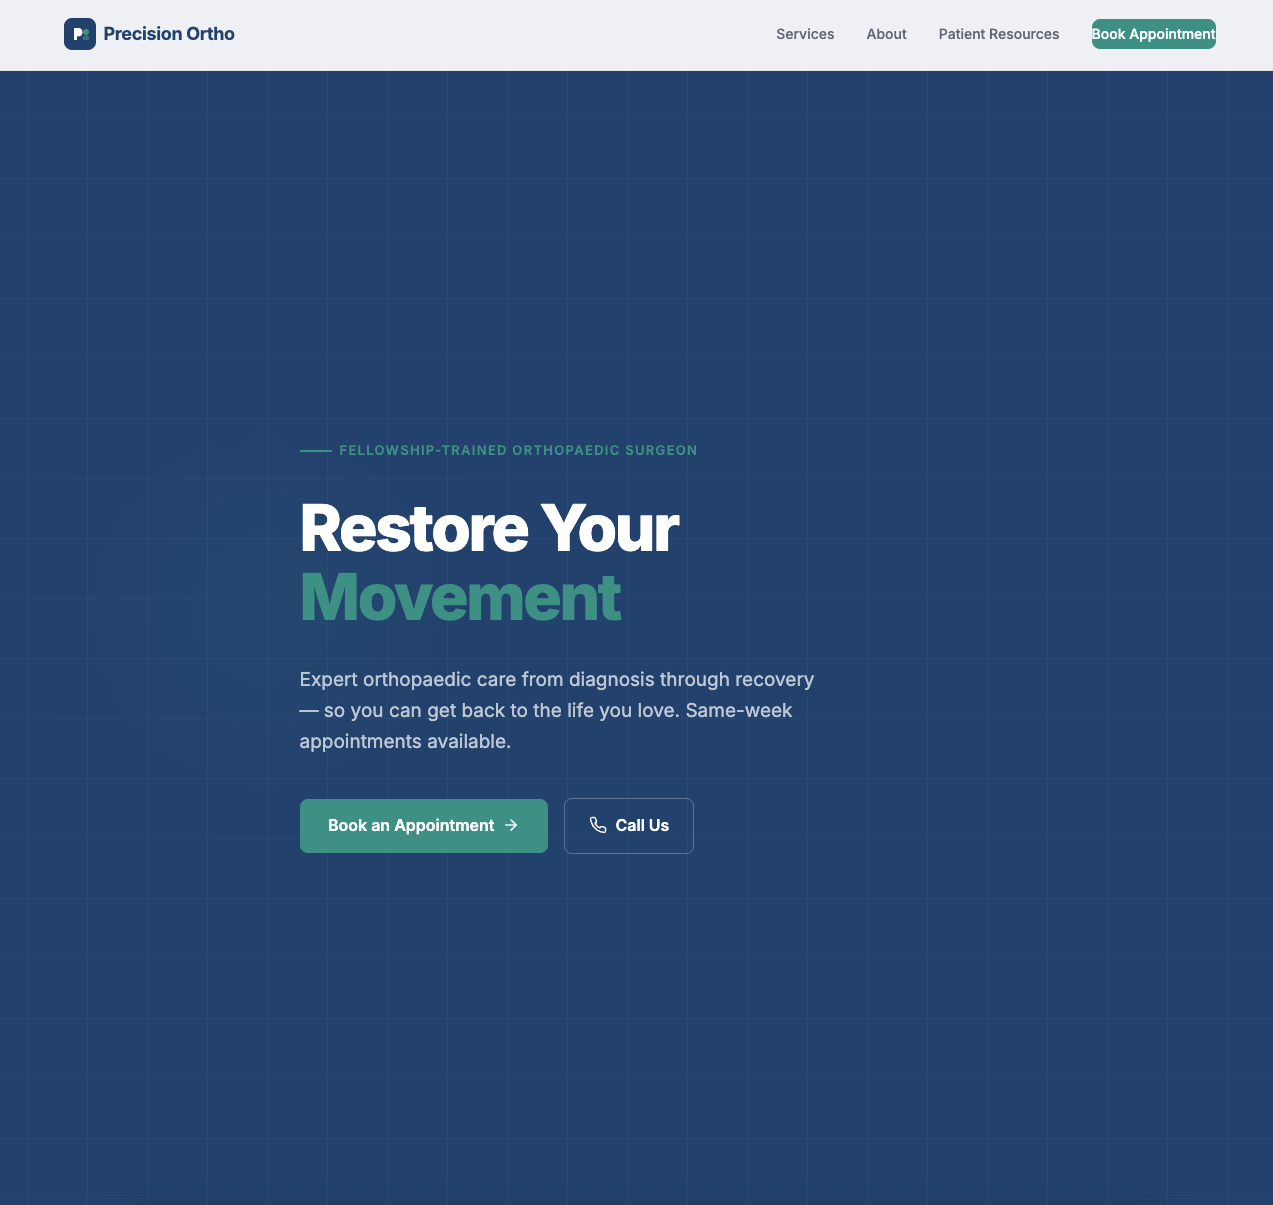
\includegraphics[width=\linewidth]{screenshots/skill-desktop.png}\\
{\scriptsize (a) Skill}
\end{minipage}\hfill
\begin{minipage}{0.32\textwidth}
\centering
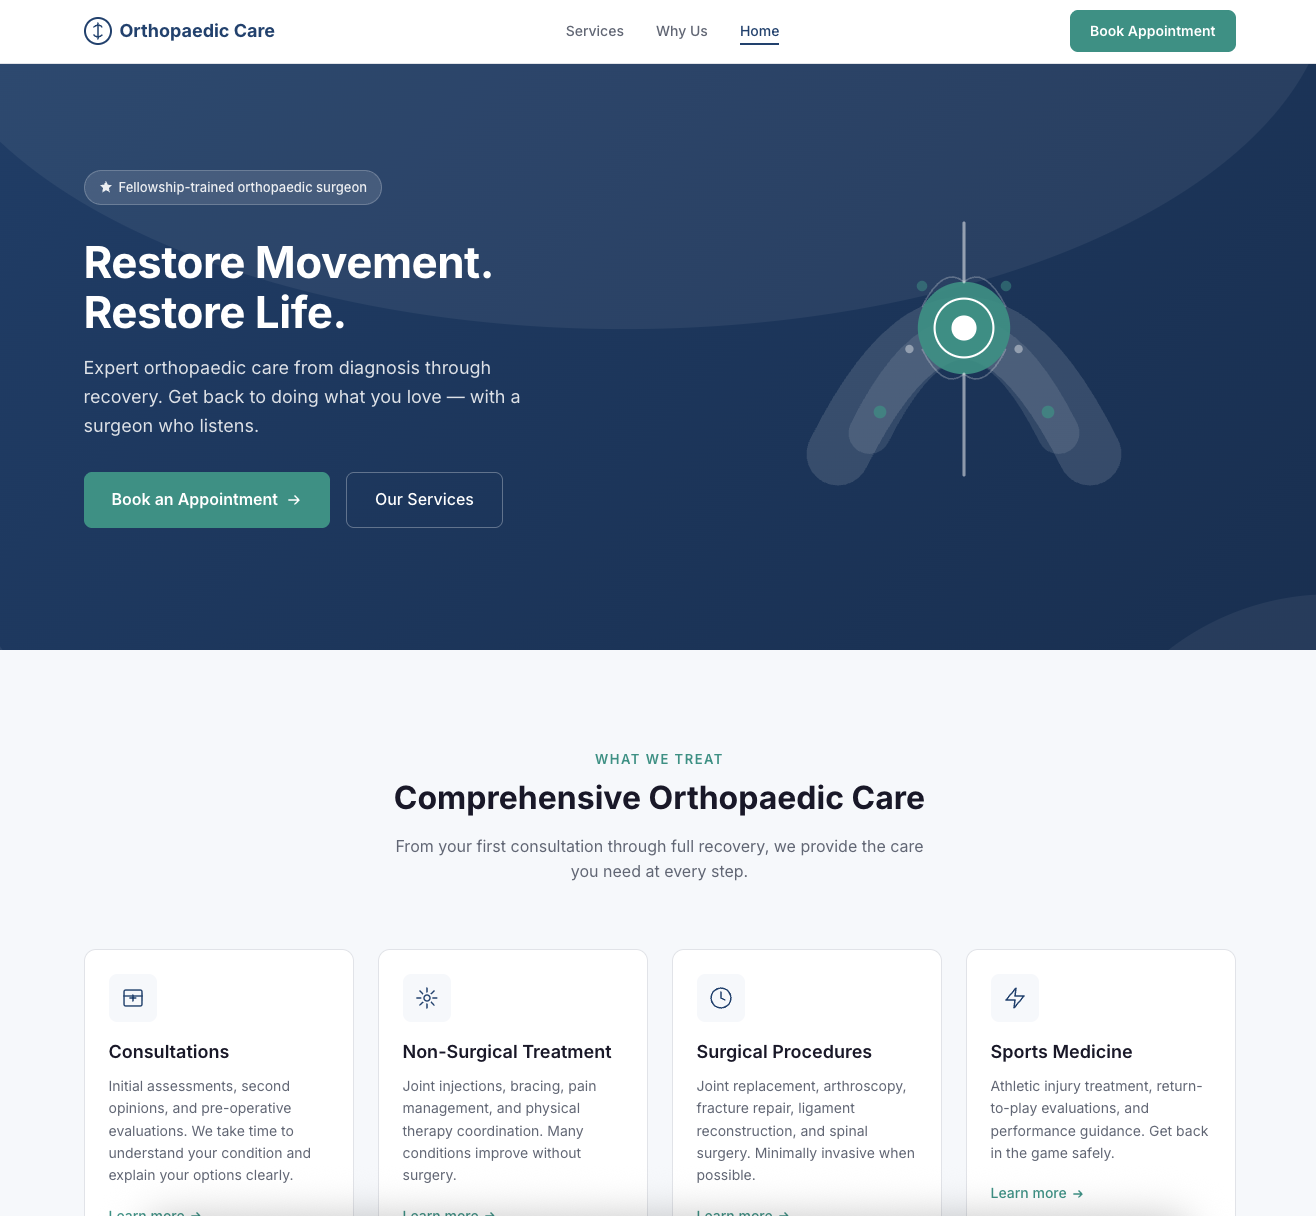
\includegraphics[width=\linewidth]{screenshots/workflow-desktop.png}\\
{\scriptsize (b) Workflow}
\end{minipage}\hfill
\begin{minipage}{0.32\textwidth}
\centering
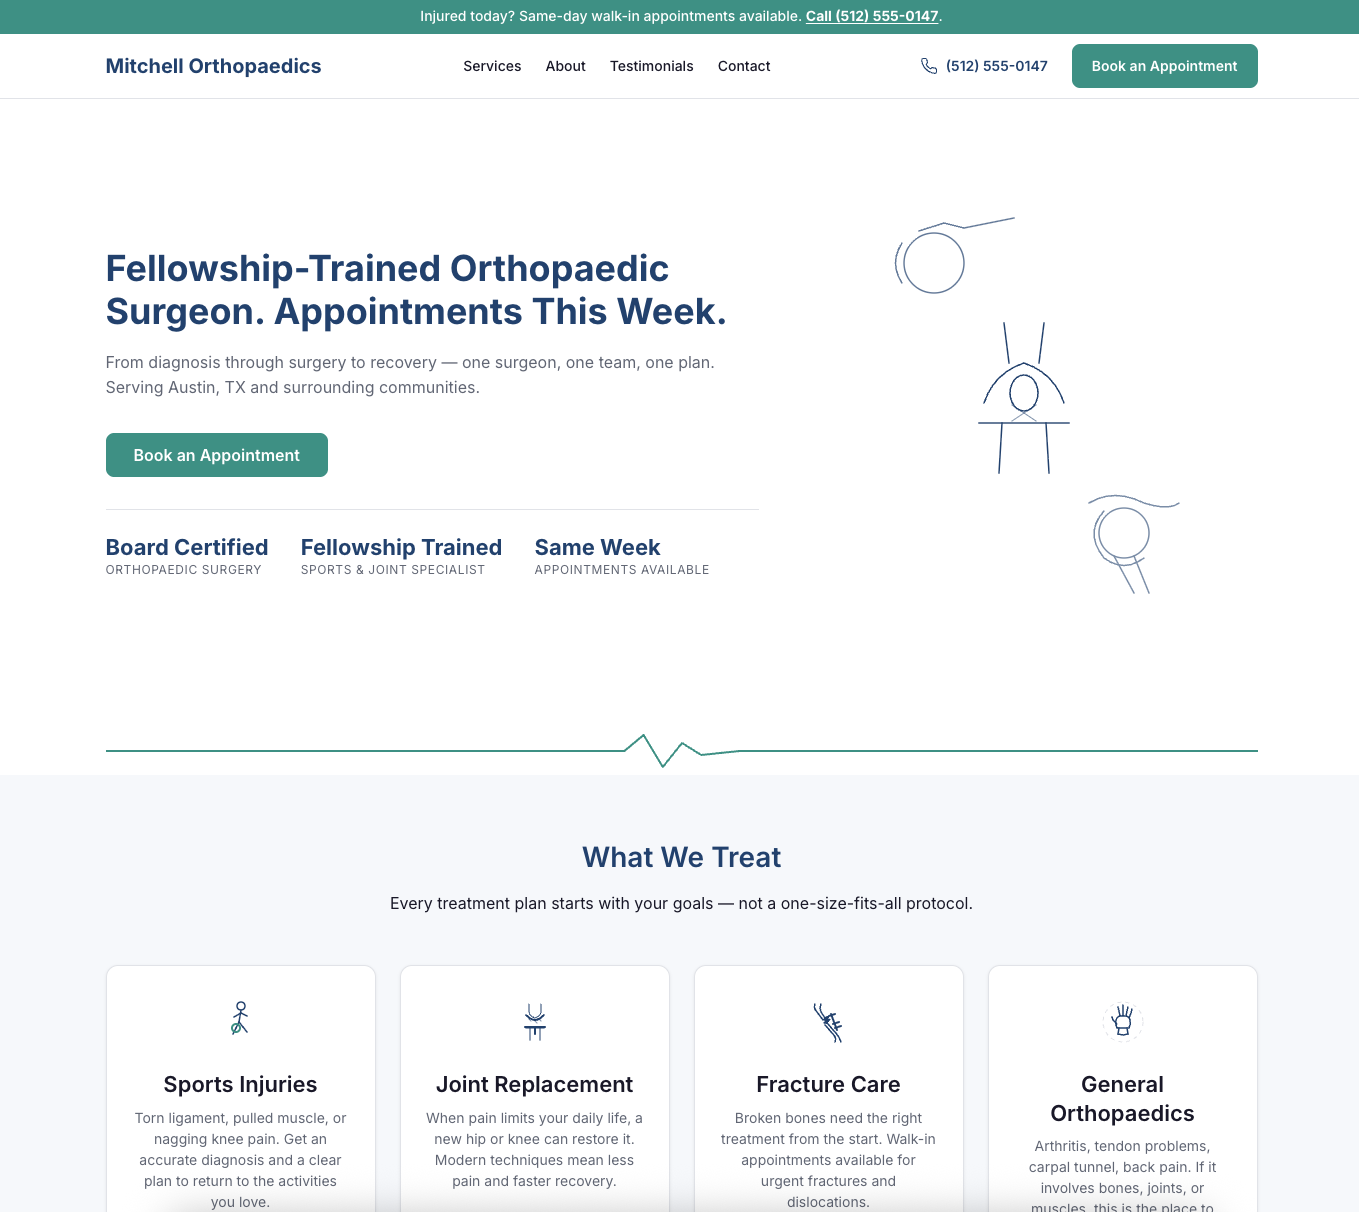
\includegraphics[width=\linewidth]{screenshots/studio-desktop.png}\\
{\scriptsize (c) Creative studio (final)}
\end{minipage}
\caption{Desktop hero sections. The skill (a)~shows ``Precision Ortho'' with no
surgeon name or location; the workflow (b)~uses ``Orthopaedic Care'' with
generic icons; the creative studio (c)~displays ``Mitchell Orthopaedics'' with
an urgent-care banner, phone number, location, credentials, and custom
anatomical SVGs.}
\label{fig:desktop}
\end{figure}

\subsection{Persona Coverage}

Table~\ref{tab:coverage} records how each output addresses the documented needs
of the three personas.\footnote{The 12 needs correspond to feature rows in
Table~\ref{tab:coverage}, each traceable to a statement in the ICP, derived
before examining outputs; a different granularity would change the magnitude of
the difference.} The skill covers 1 of 12 needs, the workflow 0, and the
studio's R1 build 1 --- comparable to the skill despite a dedicated copywriter
and designer. The final R2 build covers 10 of 12; the jump from 1/12 to 10/12
occurred entirely through the feedback loop.

\begin{table}[ht]
\caption{Persona need coverage by approach.}
\label{tab:coverage}
\centering
\small
\begin{tabular}{>{\raggedright\arraybackslash}p{5.2cm}>{\centering\arraybackslash}p{1.2cm}>{\centering\arraybackslash}p{1.4cm}>{\centering\arraybackslash}p{1.1cm}>{\centering\arraybackslash}p{1.2cm}}
\toprule
Patient need & Skill & Workflow & CS R1 & CS R2 \\
\midrule
Online booking mechanism & No & No & No & Yes \\
Surgeon credentials visible & Partial & Partial & Partial & Yes \\
Compare-and-choose info & No & No & No & Yes \\
Surgeon name and face & No & No & No & Name\footnotemark \\
Hospital affiliation & No & No & No & Yes \\
Insurance information & No & No & No & Yes \\
Phone path with equal weight & Partial & No & Partial & Yes \\
Empathy for surgical anxiety & No & No & No & Yes \\
Same-day availability above fold & No & No & No & Yes \\
Walk-in information & Partial & No & Partial & Yes \\
Practice address & No & No & No & Yes \\
Saturday hours & No & No & No & Yes \\
\textbf{Total needs addressed} & \textbf{1/12} & \textbf{0/12} & \textbf{1/12}
& \textbf{10/12} \\
\bottomrule
\end{tabular}
\end{table}
\footnotetext{No approach can provide a surgeon photograph, because none exists
in the reference documents --- a hard constraint shared by all approaches.}

\subsection{Conversion Path Analysis}
\label{subsec:conversion}

A medical homepage has one job: get the patient to book or call. The
\textbf{skill} hero CTA links to \texttt{\#contact} $\rightarrow$ another CTA
linking to \texttt{\#} (a dead end); its phone CTA uses a reserved 555 number
that cannot reach a real practice. The \textbf{workflow} CTA links to
\texttt{\#book} $\rightarrow$ another dead-end \texttt{\#}. The \textbf{studio
R1} CTA links to \texttt{\#booking}, the \texttt{id} of the section containing
the CTA itself --- a self-referencing anchor. All three thus offer \textbf{zero
conversion paths that reach a real destination}. The \textbf{studio R2} CTA
links to \texttt{\#contact}, scrolling to an appointment-request form (name,
phone, reason) with a client-side handler that shows a confirmation but
transmits no data, alongside a \texttt{tel:} link that initiates a real call:
one interactive path (a client-side prototype) and one functional phone path.
The form was added post-evaluation in response to the Round~2 review's top P1
finding; the R2 scores in Table~\ref{tab:scores} therefore reflect the pre-form
build.

\subsection{Isolating the Feedback Loop's Contribution}
\label{subsec:isolating}

The Round~1 review isolates the feedback loop's contribution from multi-agent
generation (Table~\ref{tab:scores}). The R2 average of 7.2 falls below the
8/10 re-iteration threshold; the orchestrator addressed the top P1 finding as a
targeted fix rather than a full third iteration. Because the scoring agent also
flagged the R1 deficiencies, the deltas are evidence that flagged gaps were
addressed, not independent quality assessments.

\begin{table}[ht]
\caption{Creative studio evaluation scores across two rounds, averaged across
three personas (range in parentheses). R2 reflects the pre-form build.}
\label{tab:scores}
\centering
\small
\begin{tabular}{lccc}
\toprule
Dimension & Round 1 & Round 2 & Delta \\
\midrule
Visual & 6.3 (6--7) & 7.7 (7--8) & +1.3 \\
Copy & 7.3 (7--8) & 8.0 (8--8) & +0.7 \\
Flow & 5.7 (5--6) & 6.7 (6--7) & +1.0 \\
Conviction & 4.7 (4--5) & 7.0 (7--7) & +2.3 \\
Persuasion & 4.7 (4--5) & 7.0 (6--7) & +2.3 \\
\textbf{Average} & \textbf{5.7} & \textbf{7.2} & \textbf{+1.5} \\
\bottomrule
\end{tabular}
\end{table}

The five P1 bounce triggers common to all three personas were a
self-referencing CTA, a placeholder surgeon name, an obviously fake phone
number, no practice name/address/hours/location, and no header or footer ---
exactly the gaps in the skill and workflow outputs. Despite a dedicated
designer and copywriter, the studio's R1 build had \textbf{identical
content-completeness failures} to the single-agent approaches; multi-agent
generation improved copy quality (R1 scored 7.3 on Copy) and visual consistency
(custom anatomical SVGs over generic feather icons), but added none of the
distinguishing content. The additions between R1 and R2 --- testimonials,
hospital affiliation, insurance, urgent-care banner, empathy line, hours, real
address --- were each traceable to specific customer findings, and the largest
gains fell in Conviction (+2.3) and Persuasion (+2.3), the dimensions most tied
to that content.

\subsection{Qualitative Differences}

\textbf{Copy.} The skill and workflow hero subtitles are competent but generic
(``get back to the life you love''), interchangeable with any practice. The
studio's reads ``From diagnosis through surgery to recovery --- one surgeon,
one team, one plan. Serving Austin, TX and surrounding communities,'' with
specificity and location decided in the designer--copywriter brainstorm.
\textbf{Service icons.} Skill and workflow use generic feather-style SVGs
(Fig.~\ref{fig:desktop}a--b); the studio uses custom anatomical SVGs per
service (Fig.~\ref{fig:desktop}c). \textbf{Persona-specific features.} Only the
studio's final output has segment-specific features. The urgent-care banner
(Fig.~\ref{fig:mobile}c) exists because the agent, as an acute injury patient,
wrote: ``I am sitting in an ER with a broken wrist and the first thing I see is
`Appointments This Week.' This week? I need to be seen today.'' The empathy line
exists because the agent, as a 68-year-old facing joint replacement, noted the
page ``never addresses the emotional weight of considering surgery.''

\begin{figure}[ht]
\centering
\begin{minipage}{0.22\textwidth}
\centering

\includegraphics[width=\linewidth]{screenshots/skill-mobile.png}\\
{\scriptsize (a) Skill}
\end{minipage}\hfill
\begin{minipage}{0.22\textwidth}
\centering

\includegraphics[width=\linewidth]{screenshots/workflow-mobile.png}\\
{\scriptsize (b) Workflow}
\end{minipage}\hfill
\begin{minipage}{0.22\textwidth}
\centering

\includegraphics[width=\linewidth]{screenshots/studio-mobile.png}\\
{\scriptsize (c) Creative studio}
\end{minipage}
\caption{Mobile views. The creative studio output (c)~shows the urgent-care
banner with a tappable phone link above the fold --- added after the customer
agent's evaluation as an acute injury patient on a mobile device.}
\label{fig:mobile}
\end{figure}

\subsection{Cost--Quality Tradeoff and Implementation Metrics}
\label{subsec:impl}

The studio costs roughly 10x more tokens and 10x more time but is the only
approach producing a page a patient could use to book (1, 0, and 10 of 12
persona needs for skill, workflow, and studio; 0 versus 2 real conversion
paths). The gains are non-linear: the workflow's 2x cost buys better structure
but no extra content, while the studio's 10x cost produces fundamentally
different output, most of it consumed by feedback iterations rather than by
multi-agent generation alone. On implementation metrics (Table~\ref{tab:impl}),
where the studio has no structural advantage, the workflow is leanest (820
lines, 26\,KB); the studio's added content costs a 35\% larger file and roughly
double the JavaScript --- a legitimate tradeoff of completeness against
complexity.

\begin{table}[ht]
\caption{Implementation metrics. The workflow produces the leanest
implementation; bold indicates the smallest value.}
\label{tab:impl}
\centering
\small
\begin{tabular}{>{\raggedright\arraybackslash}p{4.6cm}>{\centering\arraybackslash}p{1.6cm}>{\centering\arraybackslash}p{1.8cm}>{\centering\arraybackslash}p{2.2cm}}
\toprule
Metric & Skill & Workflow & Creative Studio \\
\midrule
Code volume (lines) & 1{,}217 & \textbf{820} & 1{,}648 \\
File size (bytes) & 39{,}124 & \textbf{26{,}125} & 53{,}869 \\
CSS custom properties & 13 & 12 & 18 \\
Inline JS (approx.\ lines) & \textasciitilde40 & \textasciitilde20 & \textasciitilde80 \\
\bottomrule
\end{tabular}
\end{table}

\section{Qualitative Analysis and Limitations}
\label{sec:analysis}

\textbf{Why feedback loops were the differentiator.} Methodology alone prevents
obvious errors --- all approaches use tokens correctly, are responsive, and
support reduced motion --- but cannot add perspectives the agent lacks; a single
builder cannot simultaneously be a 68-year-old patient facing knee replacement.
Structured thinking helps, but an agent brainstorming with itself stays within
its own boundaries. Grounded feedback was the multiplier: the customer agent
surfaced gaps no methodology or brainstorming reached, because they require a
perspective the creating agents lack.

\textbf{Grounding makes feedback actionable.} The broken-CTA finding above is
actionable because it names the technical failure (a self-referencing anchor),
states the behavioural consequence (closing the tab), establishes competitive
context (rivals have online scheduling), and implies the fix --- where a generic
``the CTA could be improved'' would not. The studio reaches multiple
perspectives through role separation (copywriter, designer, customer,
developer) that are adversarial in a productive sense: the customer agent's job
is to find what is wrong, not validate what is right. Structured thinking is
necessary but not sufficient --- the workflow produces \emph{better structure
around the same shallow content}. The practical heuristic is to \textbf{match
architecture to stakes}: methodology injection for prototypes, workflow
pipelines for production features, and the studio for high-stakes,
customer-facing pages where the 10x cost buys content that addresses real fears
rather than incremental polish.

\textbf{Limitations.} The evidence is a single instance --- one prompt, one
domain, one model, each run once --- so we cannot separate architectural
superiority from stochastic variation or richer-context exploitation a better
prompt could capture; this is the primary methodological limitation. We ran no
human evaluation: criteria are author-assessed from the ICP, a circularity that
prevents independent judgment and, for a user-centred study, is the most
significant gap. All agents used the same model; we ran no A/B test of
conversion; and a more detailed prompt or a thinner ICP might narrow the gap,
since we hypothesise the loop's contribution scales with persona-document
richness.

\textbf{Confounds and the need for ablation.}
\label{subsec:ablation}
The independent variable bundles three changes: number of agents, specialised
creative roles, and a grounded feedback loop. The R1 comparison suggests
multi-agent generation contributes \textbf{copy quality and visual consistency}
while the feedback loop contributes \textbf{content completeness and persona
coverage} --- but this is observational, not experimental. Four ablations would
isolate the components: (1)~a single agent with the creative direction
pre-loaded; (2)~multi-agent generation without customer feedback; (3)~a single
agent with Self-Refine-style self-evaluation using persona instructions; and
(4)~the full studio. Until then, attribution of the gains to the feedback loop
remains a supported hypothesis, not a proven mechanism.

\section{Future Work}
\label{sec:future}

We prioritise by expected impact: (1)~run the four \textbf{ablation} conditions
above to isolate each component; (2)~a \textbf{human evaluation} presenting all
three outputs (unlabelled, randomised) to UX designers and persona-matched
participants performing a booking task; (3)~a low-cost \textbf{minimal
replication} re-running the skill approach to test whether the content gap is a
single-run artifact; (4)~a \textbf{full replication} (five runs per
architecture, two additional domains) reporting mean and variance on persona
coverage; (5)~\textbf{prompt-specificity} experiments; and (6)~\textbf{cost
optimisation} via hybrid architectures that add a single grounded evaluation
pass to cheap generation.

\section{Conclusion}
\label{sec:conclusion}

Holding constant the prompt, model, design system, and reference documents, we
found that skill architecture --- not model capability, prompt engineering, or
design system completeness --- was the primary determinant of output quality in
this instance. The critical differentiator was not the number of agents or the
token volume but \textbf{grounded evaluation}: a customer agent that adopts
specific personas, scores against a consistent rubric, and ties findings to
observable behaviours. The studio's pre-feedback output shared the single-agent
content gaps; the additions emerged only after persona-grounded evaluation
flagged them as bounce triggers. For high-stakes, customer-facing deliverables,
the 10x investment produced non-linear gains --- fundamentally different
content, not incremental polish. Methodology prevents bad output, structure
produces good decisions, and feedback loops produce the right decisions.
Whether this generalises beyond the single domain, model, and prompt tested here
requires the proposed replication, ablation, and human evaluation.

\section{Ethical Considerations}
\label{sec:ethics}

The studio output contains fabricated medical content: ``Dr.~Sarah Mitchell,
MD'' and ``Mitchell Orthopaedics'' are fictional. ``St.~David's Medical
Center'' is a real Austin institution; its use in a fictional context is noted
as a limitation. The phone number uses the reserved 555 exchange to prevent
accidental calls, and the address is fictional. None of the generated pages
were deployed, indexed, or made publicly accessible. LLM-generated medical
content that blends real and fictional entities risks patient deception if
deployed without verification; we recommend mandatory human review before
publication, clear labelling of generated content during development, and
verification that no real patient could mistake a prototype for an operational
practice. The energy cost of 500K+ tokens per page is a further consideration
for adoption at scale. The authors declare no competing interests.

% Tighten reference-list spacing to keep the bibliography compact.
\let\OLDthebibliography\thebibliography
\renewcommand\thebibliography[1]{%
  \OLDthebibliography{#1}%
  \setlength{\itemsep}{1pt}%
  \setlength{\parsep}{0pt}%
}
\bibliographystyle{splncs04}
\bibliography{references}

\end{document}
